\chapter{Histoire de la présence musulmane en France}
\mn{LUNDI 8 NOVEMBRE 2021 (1
er cours)}


\section{Introduction}


\begin{quote}
    «{Supposez qu’il se crée en France non pas un islam français, mais un islam de France, disons pour simplifier, un islam gallican,} c’est-à-dire un islam qui soit au fait des préoccupations d’une société moderne, qui résolve les problèmes qu’il n’a jamais eu à résoudre dans ses sociétés d’origine qui, pour des raisons historiques, ne sont pas des sociétés du niveau du nord de la Méditerranée. Figurez-vous le retentissement qu’aurait cet islam de progrès sur le reste de la zone islamique»  \sn{(Berque et Sur, 1996. 25-26) Berque est le premier des islamologues français quittant l'orientalisme précédent. }: .

\end{quote}

Ce qui nous intéresse ici, ce sont les termes : 
\bi
\item \textbf{Islam en France} : les premiers contacts; Eléments d’histoire de la présence musulmane en France : Moyen-Age, soldats
nord-africains (période coloniale), 
\item \textbf{Islam de France} : Grande mosquée de Paris, et immigration de
travail.
\item \textbf{Islam Français} : plus récent, en construction, un islam qui intègre les spécificités françaises

\ei
% -------------------------------------------------------------------
\section{Premiers contacts (Moyen-Âge, Septimanie, Fraxinet, Moussais/Poitiers…)}



\paragraph{Les incursions dans le Sud de la France (Septimanie/Narbonne) – 719-759}

\paragraph{732 - bataille de Poitiers} Marque la défaite des ducs d'Aquitaine. D'autres incursions sarrasines auront lieu. 


\paragraph{Le «Massif des maures» (Fraxinet) entre 850 et 973}
 
 \begin{marginfigure}
    \centering
    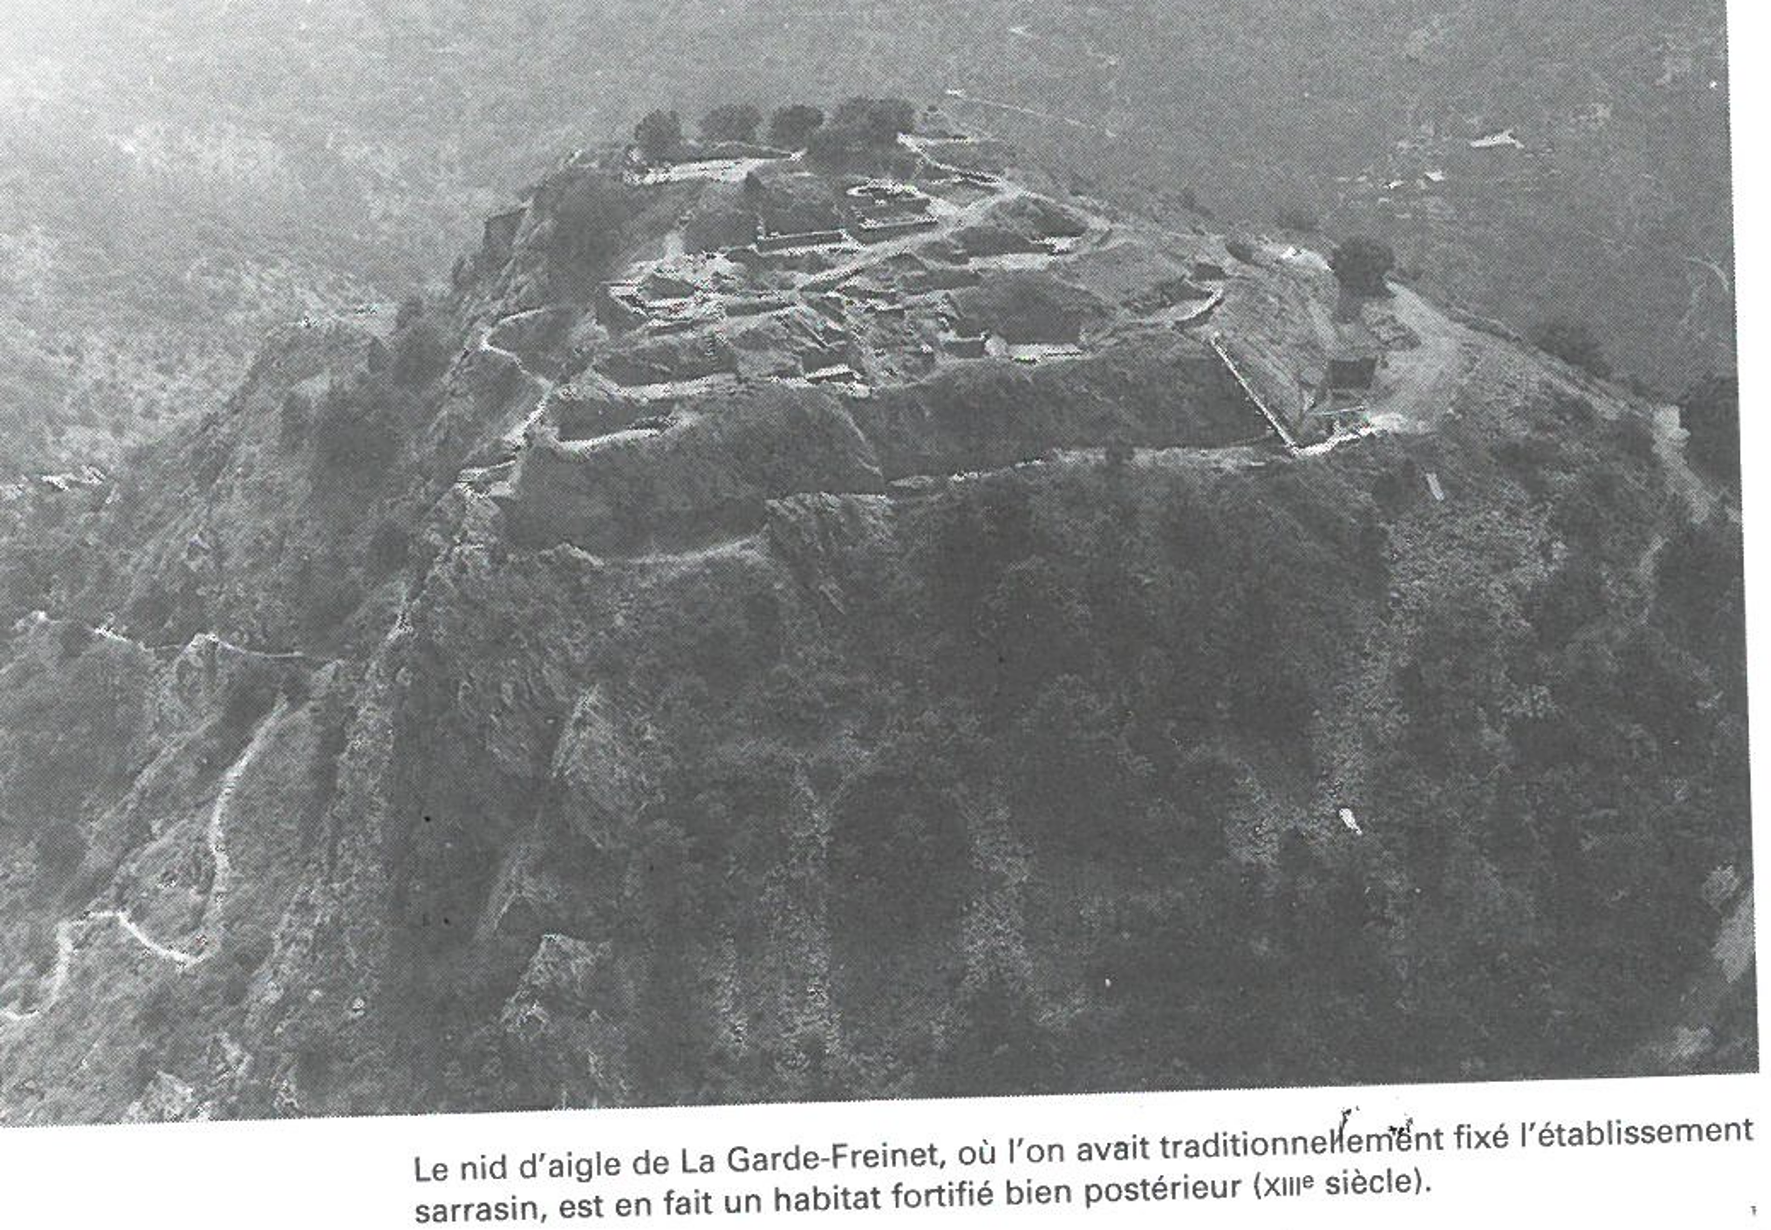
\includegraphics[width=\textwidth]{Images/nidAigle.png}
    \caption{Le nid d'aigle}
    \label{fig:nidAigle}
\end{marginfigure}

 Fraxinet ou Fraxinetum est un établissement pirate puis comptoir  sarrasin du xe siècle dans le golfe de Saint-Tropez, dans le Var. Le territoire de la cité, aux limites mal définies (peut-être la commune actuelle de La Garde-Freinet), est conquis par des marins venus d'Al-Andalus vers 890 et repris par le comte de Provence Guillaume Ier (surnommé ensuite « le Libérateur ») en 973 après la bataille de Tourtour.
 

\begin{figure}[h!]
    \centering
    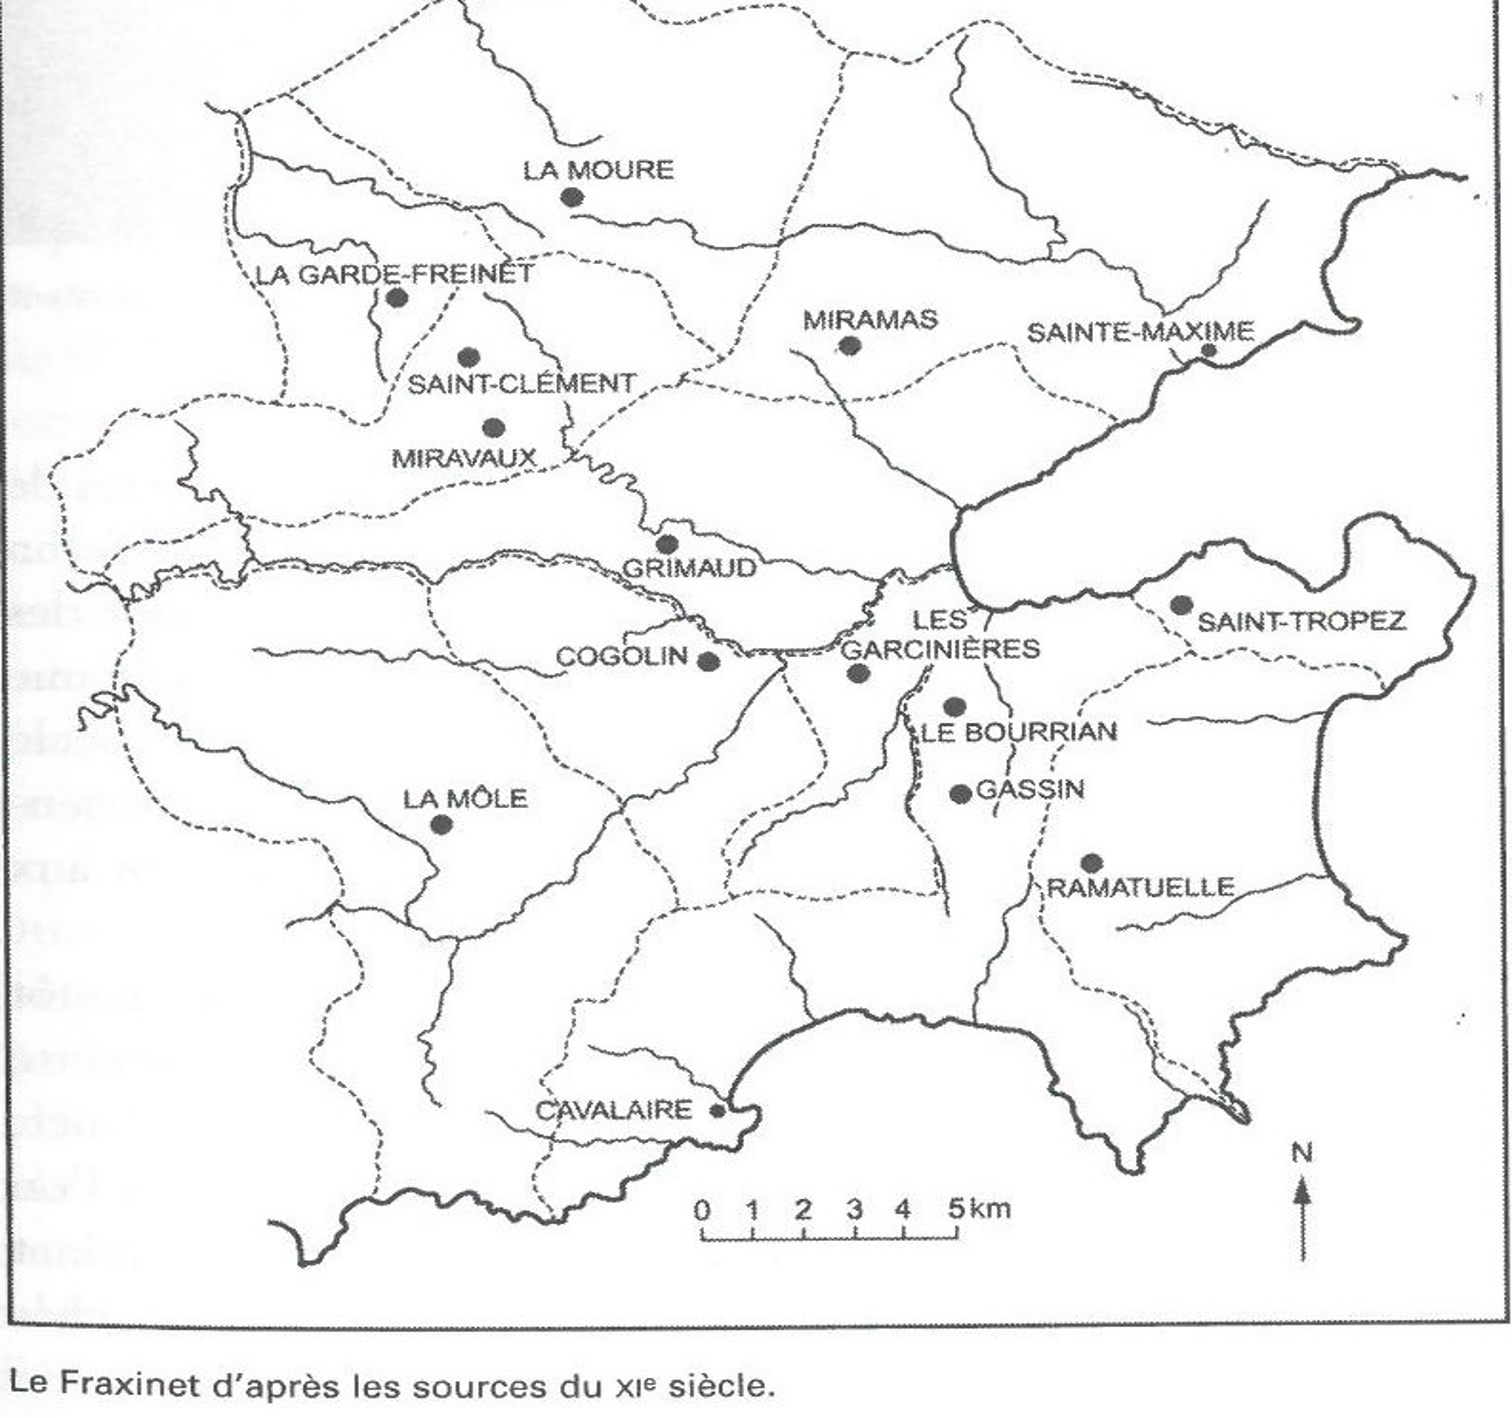
\includegraphics[width=\textwidth]{Images/Fraxinet.png}
    \caption{Le « Massif des maures » (Fraxinet) }
    \label{fig:Fraxinet}
\end{figure}

\paragraph{Des tombes musulmanes du début du Moyen-Âge à Nîmes (2016)} confirment cette présence. Abbé Liut avait confirmé cette présence.

3 sépultures à Nîmes avec une posture de corps du côté droit et le regard vers le sud est (direction de la Mecque). Un surcreusement pour placer le corps. Grâce à des analyses paleo-génétiques, des marqueurs du nord de l'Afrique.

\paragraph{Découverte récente (en Espagne)}

400 tombes découvertes dans la province de Saragosse orientées vers la Mecque, certainement des premières générations de musulmans installés dans la péninsule suite au débarquement de Tarik Ibn Zyad en 711. Probablement des \textit{convertis à l'islam, mais qui ont une culture traditionnellement romaine, donc ils apportent la preuve d'un moment de transition culturelle}.


\paragraph{Les Croisades, 1095-1291}
lancées par le pape Urbain II depuis Clermont.
période de rencontre entre Orient et Occident.

\paragraph{Autres événements}
On peut évoquer des accords diplomatiques : 1536 François 1er et Suliman le Magnifique : capitulations et installation des Echelles dans le Levant.

\paragraph{Des échanges plus pacifiques et culturels} \href{https://fr.wikipedia.org/wiki/Arnoult_de_Lisle}{Arnoult de Lisle}, médecin, apprend l'arabe pour lire Avicenne. 1587, première chaire d'Arabe. Il vit 11 ans au Maroc et retourne ensuite comme envoyé d'Henri IV.
1610 : Henri IV accueille plus de cent milles de musulmans chassés d'espagne (morisques). \sn{\href{https://www.culture-islam.fr/contrees/maghreb/henri-iv-de-bourbon-ordonnance-concernant-laccueil-et-le-transfert-des-morisques-despagne-22021610}{l'ordonnance d'Henri IV} autorisant le passage des morisques}

1884 : influence de la France en Orient. Muhammad ‘Abduh, egyptien, futur grand mufti d'Egypte, chassé par les oulémas conservateurs, fonde la revue \emph{al-‘Urwa al-wuthqa} ou "le lien indissoluble" à Paris avec Jamal al-Din al-Afghani, véritable fondateur du réformisme moderne \sn{\url{https://www.lesclesdumoyenorient.com/Jamal-al-Din-al-Afghani-fondateur.html}}.



%------------------------------------------------------------------------
\section{Sujets coloniaux, soldats, travailleurs, puis citoyens}


\subsection{La présence musulmane en France : rappels historiques}


Avec la conquête de l'Algérie en 1830 débute la présence coloniale de la
France dans des pays de population musulmane. La colonisation de
l'Afrique occidentale française, de l'Afrique équatoriale française, les
protectorats du Maroc et de la Tunisie, la présence durable de la France
en Algérie organisée en trois départements ou les mandats du
Moyen-Orient (Syrie et Liban) ont placé \emph{de facto} pendant près
d'un siècle des pays musulmans sous gouvernance et administration
françaises. Selon les périodes, des millions de musulmans d'Afrique, du
Maghreb, du Moyen- Orient et de l'Océan indien furent français, avec
différents degrés de citoyenneté, théorique ou effective.

La présence de musulmans sur le territoire métropolitain est plus
circonscrite dans le temps : elle commence au début du XXe siècle, même
si elle ne concerne alors que quelques milliers d'individus. Pendant la
Première Guerre mondiale, la France mobilise ses « troupes coloniales »,
600 000 hommes, dont les goumiers marocains et les tirailleurs
sénégalais ; mais aussi presque un tiers de la population masculine
algérienne âgée de 20 à 40 ans. Cette première présence musulmane sur le
territoire métropolitain ne se limite pas aux troupes, puisqu'à
l'arrière de nombreux musulmans travaillent dans les usines régies par
le Service d'Organisation des Travailleurs Coloniaux, qui dépend de
l'armée. L'État institue la carte de séjour en 1917 et c'est à partir de
l'entre-deux-guerres qu'il prend en charge cette immigration, et en
particulier l'immigration nord-africaine. Il crée aussi les brigades des
affaires nord-africaines, rattachées au ministère de l'Intérieur et des
Affaires sociales. Cette première présence musulmane se lit par quelques
bâtiments symboliques, tels que la Mosquée de Paris, inaugurée par le
président Gaston Doumergue en 1926 aux côtés du sultan du Maroc Moulay
Youssef, ou bien l'hôpital franco-musulman Avicenne à Bobigny en 1925.

Le Front Populaire accorde le droit de libre-circulation sur le
territoire aux Nord- Africains, sous réserve qu'ils possèdent une carte
d'identité et un visa spécial. À la fin des années 1930, la France a un
solde naturel négatif et le pays manque de main d'œuvre, si bien qu'à la
chute du Front Populaire, les naturalisations s'accélèrent et des
dérogations aux quotas d'emplois étrangers sont accordées par
l'inspection du travail.


En étant un peu plus précis : 

\paragraph{1798: Expédition d’Egypte par Napoléon}
(essor de l’Orientalisme)

\paragraph{1830: tutelle coloniale sur l’Algérie qui durera 130 ans.}
Une autre phase s'ouvre. 
Suivront l’Afrique de l’Ouest, le Maroc (« Protectorat »), la Tunisie, la Syrie-Liban. Abd El Kader a été libéré par Napoléon III en 1853 et envoyé en Syrie.




\subsection{Les musulmans dans l'armée française de 1900-1945}
{Participation de centaines de milliers de soldats nord-africains et ouest-africains aux deux guerres mondiales, au sein de l’armée française}
Certains bataillons gardent le croissant sur le béret encore aujourd'hui \sn{Régiment d'Epinal et les Spahis de Valence}.
(se forme à cet occasion les premières bases d’une proto-aumônerie militaire musulmane) 
\begin{figure}
    \centering
    \includegraphics[width=\textwidth]{Images/MosqueeFrejus.jpg}
    \caption{La Mosquée de Fréjus, édifiée en 1928 et de style malien, pour les tirailleurs sénégalais de Frejus}
    \label{fig:Frejus}
\end{figure}
\mn{Epinay sur Seine : exposition sur la présence musulmane en France}




\mn{\cite{Arkoun:histoire}}

500,000 hommes sous les drapeaux en 1914, dont 100,000 morts. Une conscription obligatoire en 1916, organisée par Gallieni : 250 000 hommes du Maghreb, avec quelques révoltes.
 
\bi
\item dans l'ensemble, reconnu pour leur combativité et bien accueilli par les populations métropolitaines. \sn{Voir à Invalides les plaques citant leur courage}
\item respect de la foi des musulmans par l'armée et en particulier des rites d'inhumation. Mais \textit{parfois le sentiment d'en faire trop; cf la prière dehors et non dans les mosquées}
\item Rôle paternaliste (sens positif) des officiers (cf Juin apprenant l'arabe dans les tranchées de 14)
\item une demande parfois exprimée pour une égalité de traitement, y compris sur le vin.
\item Pénétration du discours moderniste dans la masse musulmane (cf développement de la scolarisation). 
\item Glorifié par la poésie populaire notamment en Algérie. 
\ei



\begin{Synthesis}
Le tirailleur revient du font complètement transformés; Encadrés en permanence par des Français, les musulmans tenaient à leur prouver qu'ils étaient capables de s'adapter aux exigences de la guerre moderne et de se battre contre ceux qu'ils considéraient comme les meilleurs soldats du monde  ; les allemands. 
\end{Synthesis}
Mais le discours français sur la liberté et la justice fut repris par des nationalistes maghrébins et retourné contre la puissance coloniale. 


\paragraph{1905: fondation mosquée de St Denis de La Réunion}
(par des émigrés indiens du Gujarat)

\paragraph{Accord dès 1767 signé entre Sidi Mohammed Ben Abdallah (Roi du Maroc) et Louis XV pour une première mosquée en France}
 mais qui ne verra pas le jour.


\subsection{1926: Grande mosquée de Paris}
début du crédit accordé puis des travaux en 1920

\paragraph{tentatives avortées en 1846}
le oomte de Pommereux, répond : 
\begin{quote}
« Il m'a
toujours paru difficile de pouvoir fonder une mosquée à Paris. Les
musulmans n'ont pas deux lois, mais une seule. Si ce n'était
qu'une loi religieuse, cela aurait peu d'inconvénients; mais c'est
en même temps une loi civile, opposée au principe même de notre
constitution, ce qui pourrait devenir pernicieux, parce que l' on ne
peut pas séparer l'une de l'autre. D'ailleurs, vous connaissez
l'esprit anti-progressif, intolérant du Koran. Et puis, écrit, rédigé
pour un peuple nomade, qui avait besoin de trouver sous sa main
la solution des questions civiles et religieuses, il ne convient plus
aussi bien à des populations stables. »
\end{quote}
La réaction du ministère de la Justice et des Cultes est~négative parce que les musulmans sont en faible nombre et ne l'ont pas demandé.

Un édifice au père lachaise est construit en 1857 pour le soins des défunts et leurs funérailles.

\paragraph{Un exemple de converti au XIXeme : Philippe Grenier}
Image d'un homme aux convictions sincères mais le caractère ostentatoire des prières en public semble avoir ridiculisé .
\begin{marginfigure}
    \centering
    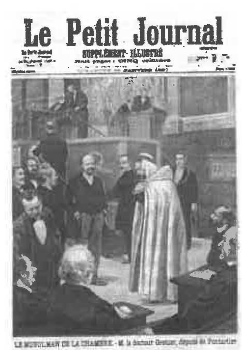
\includegraphics[width=\textwidth]{Images/DocteurGrenier.png}
    \caption{le docteur Grenier converti à l'islam à la chambre des députés, \textit{le Petit Journal} 24 Janvier 1817.}
    \label{fig:DocteurGrenier}
\end{marginfigure}
Il assiste à l'inauguration de la mosquée de Paris en 1926.

\paragraph{La société des Habous à la Mecque}
autre impulsion conduisant à la création de la Mosquée de
Paris est la mise en place, par le Quai d'Orsay, de la Société des
habous en 1916-1917. Celle-à est liée à la diplomatie de guerre
menée par la France au Proche-Orient. Pour contrer les menaces
sur les colonies à population musulmane que l'appel du calife au
\emph{jihâd} fait peser, la France a contracté une alliance avec le cherif
Hussein de la Mecque qui déclenche la révolte arabe contre les
Turcs dam le Hedjaz le 10 juin 1916. C'est la grande mission de
\emph{Si Kaddour Ben Ghabrit }(186~-1954), un Algérien entré au service
de l'administration du protectorat au Maroc en 1892 et
agent diplomatique français de grande envergure.
Le chef du gouvernement Aristide Briand, envoie Ben Ghabrit à
la tête d'une délégation de pèlerins nord-africains après avoir
décidé la réouverture du pèlerinage de La Mecque le 2 août 1916.
Dans le but de pérenniser la présence française, il est statué finalement
sur 1a question de l hôtellerie des pèlerins à la Mecque.
Celle-ci avait été évoquée en 1915 par la Commission interministérielle
des affaires musulmanes mais le gouvernement Général
de l'Algérie s'y était opposé. De la même manière il s'oppose
au projet de « Village kabyle » comprenant notamment une mosquée.
envisagé par la chambre de commerce de Marseille en
1917. Mais le Parlement vote un crédit de 500000 francs le
31 janvier 1916 et Pierre de Margerie (1861-1942), ancien secrétaire
général de la conférence d'Algesiras pour le Maroc (1906)
et directeur des Affaires politiques au Quai d'Orsay pendant toute
la guerre, organise le dispositif exécutoire qui débouche sur
l'achat d'un bâtiment à La Mecque et la création de 1a Société des
habous comme organisme propriétaire et administrateur.
Seul-un bien habous, en effet, c'est-à-dire une propriété de type
religieux inaliénable, insaisissable et imprescriptible, autorisait
la détention indirecte par le gouvernement français d'un bien
immobilier dans l'enceinte de La Mecque. Et un tel bien habous
devait être administré par une \textit{Société des habous} (on dirait
aujourd'hui une association). C'est Pierre de Margerie qui en
désigne lui-même les membres, parmi lesquels Si Kaddour Ben
Ghabrit qu'il charge de la présidence de la commission chargée de la création. 

La mosquée est financée par l'Etat.

\begin{Synthesis}
On voit comment
s'imbriquent le devoir religieux qui incombe à la France en tant
que puissance musulmane et les impératifs diplomatiques.
Cette société des Habous est encore propriétaire des lieux de la Mosquée de Paris
\end{Synthesis}

\paragraph{Loi française et inspiration marocaine : l'institut musulman}
Edouard Herriot, partie radical, à la suite de l'effort de guerre de la main d'oeuvre venus des colonie, a un respect de libre penseur pour l'Islam : "Encourageons cet islam qui s'éveille ou se réveille". En 1920, il fait voté 500 000 francs pour la mosquée de Paris "vraie maison de l'Islam".

Il est étonnant de noter qu'après la loi de séparation de l'Eglise et l'Etat, une telle subvention ait pu être votée. Un sénateur, Dominique Delahaye, note : "puisqu'on parle des musulmans, il serait bientôt temps de traiter les catholiques aussi bien que les musulmans".

L'architecte choisi est Maurice Tranchant de Lunel, appartenant à l'entourage Lyautéen de Rabat et qui a beaucoup voyagé. La mosquée s'inspire de l'architecture marocaine, mais aussi de l'Espagne d'al Andalus et de l'Inde musulmane. 

A leurs côtés,
Maurice Co1rat représente le gouvernement. Il est l'auteur de
1a fameuse formule, attribuée parfois à tort à Lyautey :
\begin{quote}
    « Quand
il s' érigera, au-dessus des toits de la ville, le minaret que vous
allez construire à cette place, il ne montera vers le beau ciel
nuancé de l'Île-de-France qu'une prière de plus, dont les tours
catholiques de Notre-Dame ne seront point jalouses. »
\end{quote}

L'inauguration de la Mosquée de Paris a lieu le 15 juillet 1926 en présence du président Gaston Doumergue et du sultan du Maroc. Le discours de Si Kaddour Ben Ghabrit 
\begin{quote}
    
Ma confusion le dispute à
ma fierté de voir ici réunis le plus haut représentant de la nation
~ et Sa Majesté le sultan du Maroc. Cette réunion est symbolique. Elle marque que 1a France, fidèle à une politique plusieurs
fois sécu1aire affirme d'éclatante manière la sympathie qu'elle ressent pour les musulmans de toutes origines qui sont pour elle également des amis. Cet hommage de haut et noble libéralisme aura, a déjà eu le plus grand retentissement dans le monde musulman car il démontre que la France hospitalière à toutes les races ne l'est pas moins à toutes les idées, à toutes les religions. \end{quote}

Gaston Doumergue n'hésite pas à citer un \emph{hadith} du Prophète consistant à définir le meilleur islam : 
\begin{quote}
    c'est celui du croyant dont les musulmans n'ont à redouter ni la main ni la langue
\end{quote}
et à conclure : "cet islam-là est aussi le notre".


il y eu des réactions comme Charles Maurras : 
\begin{quote}
    Cette mosquée en plein Paris ne me dit rien de
bon. Il n'y a peut être pas de réveil de l'islam, auquel cas tout ce
que je dis ne tient pas et tout ce que l'on fait se trouve être la plus vaine des choses. Mais, s'il y a un réveil de l'islam, et je ne
crois pu que l'on en puisse en douter, un trophée de la foi coranique sur cette colline Sainte-Geneviève où tous les plus grands docteurs
de la chrétienté enseignèrent contre l'islam ~ plus
qu'une offense à notre passé : une menace pour notre avenir. 
\end{quote}

\paragraph{Sous le giron Algérien}
Si la Grande mosquée de Paris est d'abord en effet sous girons français, l'indépendance de l'Algérie, une application plus serrée de la loi de 1905 qui interdit à l'Etat français de diriger un culte, et les liens diplomatiques entre les deux pays vont en effet constituer autant de facteurs qui feront passer la GMP sous le girons algérien. 

\paragraph{Rôle de contrôle de l'Islam en France} La grande mosquée a aussi pour rôle de réguler l'Islam en France, après la décolonisation. "fonction sociale implicite religieuse diaspora religieuse venant d'Algérie" \sn{Travaux de Dorra Mameri-Chaambi \href{http://www.theses.fr/2016EPHE5090}{Thèse}}
La Mosquée de Paris a participé aux différents
processus de régulation de l’islam en France, à
savoir la Commission des Six sages, le Conseil
de réflexion sur l’islam de France (CORIF) de
Pierre Joxe, la Charte du culte musulman initiée
par Charles Pasqua mais aussi l’\emph{Istichara}, c’est à
dire « la consultation » puisque le nom a été
arabisé, sous l’égide de Jean-Pierre
Chevènement, et enfin le Conseil français du
culte musulman (CFCM) à partir de 2003.

\paragraph{Le projet Blum Viollette}
Le projet de loi relatif à l'exercice des droits politiques par certaines catégories de sujets français en Algérie, dit le projet Blum-Viollette (1936), fut un projet de loi du Front populaire de Léon Blum, sur les propositions de Maurice Viollette, ancien gouverneur général d'Algérie, visant à ce que 20 000 à 25 000 musulmans puissent devenir citoyens français tout en gardant leur statut personnel lié à la religion. Le projet, délibéré en Conseil des ministres le 15 octobre 1936, est déposé sur le bureau de la Chambre des députés le 30 décembre suivant. La commission du suffrage universel l'éxamine en 1938, mais celui-ci est définitivement suspendu le 4 mars.

\paragraph{Guerre de 39-45}
340 000 hommes d'Afrique dans 14 divisions sont mobilisés en 1942-45, en particulier sous les ordres du Général Juin. Un service d'aumônerie musulmane commence à se mettre en place. On trouve même des récits d'Aid El Kebir dans l'armée. 

\mn{Consulter \emph{La France et ses Musulmans} donne la structure du plan.}



%--------------------------------------------------------------------
\section{Evolution de la présence musulmane en France (chiffres, nombre de lieux de culte…)}

\paragraph{Immigration de travail}
à partir des années 50, 
\bi
\item 200.000 «nord-africains» en 39, "une colonie nord-africaine". 
\item avec les trente glorieuses, une diversification avec beaucoup de marocains en particulier contribuant à la reconstruction. 1.600.000 «musulmans» tout pays d’origine confondus en 1985 (Krieger, 1985),
\item 1959 : premiers foyers SONACOTRA. 
\item 3,65 millions dont moitié de nationalité fra. (INED-INSEE, 2004), Michele Tribalat. \sn{1,7m d'immigrés, 1.7m d'enfants avec au moins un parent né en France, 300 000 petits enfants d'immigrés. Avec beaucoup nés en Algérie ou au Maroc.} 2.2\% de plus de 60\% mais 1 sur 10 pour les moins de 18 ans. Mais étude d'il y a 20 ans. 
\item Le prénom Mohammed est le premier prénom à Marseille en 2007.
\item L'étude \emph{TeO} INED / INSEE \sn{https://teo.site.ined.fr/}
\item 4 à 5 millions de français de confession musulmane de nos jours. français "sociologiques" indépendant de leur niveau de pratique : 1,5m d'algériens de nationalité ou d'origine, 1m de marocains, 500 000 Tunisiens, 400 000 Afrique sub-saharienne, 350 000 Turque, 70 000 du moyen orient (Liban : souvent CSP+ / Egypte : Pantin), 100 000 des Comores (école coranique en France), 250 000 de Mayotte et Réunion. Plus ou moins, fourchette. 
\ei



Après la Seconde Guerre mondiale, l'impératif de reconstruction
déclenche l'arrivée massive de populations venues de territoires de
tradition musulmane. La grande majorité des musulmans français est issue
de cette vague d'immigration, venue travailler dans les usines et les
chantiers français pendant les Trente Glorieuses. Cela explique leur
concentration sur cinq grandes zones liées à l'histoire industrielle
française :


\begin{itemize}
\item
  
  le Grand Paris, avec d'importantes concentrations en Seine-Saint-Denis
  en particulier, et un peuplement d'une grande diversité d'origines ;
  
\item
  
  Marseille et la façade méditerranéenne, dont une grande partie de la
  population est d'origine maghrébine ;
  
\item
  
  Lyon et la vallée du Rhône ;
  
\item
  
  Lille, Roubaix et le bassin minier du Nord, où prédomine la communauté
  marocaine, rifaine en particulier ;
  
\item
  
  l'Alsace, la Moselle et le bassin minier de l'Est, où la présence de
  la communauté turque est importante.
  
\end{itemize}


Depuis les années 1970 \sn{\cite{Montaigne:IslamPossible}} et le premier choc pétrolier, le flux
d'immigration de main-d'œuvre a beaucoup diminué et les musulmans qui
s'installent en France arrivent majoritairement dans le cadre du
regroupement familial. Une très large partie d'entre eux a acquis la
nationalité française, et aujourd'hui la majorité d'entre eux vit en
France métropolitaine depuis deux ou trois générations.

Les musulmans français sont dans leur majorité originaires d'Afrique du
Nord : 38 \% sont d'origine algérienne, 25 \% d'origine marocaine, 8 \%
d'origine turque et 9 \% sont originaires des pays d'Afrique
sub-saharienne. L'enquête que nous avons réalisée avec l'IFOP montre que
la très grande majorité des musulmans étrangers sont eux-aussi
originaires du Maghreb, d'Afrique ou de Turquie. Ces régions
représentent en effet 23 \% de la population totale de l'enquête et
regroupent plus de 88 \% des individus ne détenant pas la nationalité
française.


\paragraph{Regroupement familial}  (décret d’avril 1976, étendu par un arrêt du CE de 1978)

\paragraph{Lieux de Cultes}
 (approx.); 
 \bi
 
\item  autour de 100 en 1970 (on est juste avant la création des premières fédérations musulmanes dont le but sera de créer des mosquées), \item de 500 en 1985, \item de 1300 en 1992, \item de 1600 en 2003, \item de 2500 en 2014, \item autour de 3000 de nos jours (France et TOM). dont 350 dans les outre-mers, en particulier à Mayotte. \mn{280 synagogues à titre illustration}
\ei

Les différences tendances des mosquées : 
\bi
\item La tendance Marocaine (UMF, RMF) : 450 à 500 mosquées
\item La tendance Algérienne (FNGMP) : 300 mosquées
\item Fréristes (UOIF - \textit{Musulmans de France} ) : 150-200 lieux de cultes
\item Turcs (Moselle CCMTF rattaché à la Diayanet Turque) : 270 lieux  
\item Frères musulmans turcs :
Ouest Africaine (FFAI ?)  : 10 Mosquées
\item Tabligh (Foi et Pratique) : 10 mosquées
\item Salafiste : entre 100 et 200 salles Salafistes. Ne sont pas rattachés à une fédération.
\item Les 2/3 ne sont pas affiliés (Grande Mosquée de Lyon, St Ouen, Villeurbanne, ...). 
\ei


\paragraph{de sujets à citoyens}
-Sadek SELLAM (voir biblio) parle d’un passage de «sujets» (1830-1947) à «citoyens» (1947-2004).


\section{Bibliographie de la partie}
\cite{Arkoun:histoire}
KRIEGER-KRYNICKI Annie, Les musulmans en France, Maisonneuve et Larose,
1985.
SELLAM Seddak, La France et ses musulmans, Fayard, 2006.
\paragraph{Support multimédia :}
Documentaire « Nous, Français musulmans », Arte, Janvier 2020, 2 parties X 52’ :
\url{https://www.arte.tv/fr/videos/084758-001-A/nous-francais-musulmans-1-2/} et
\url{https://www.arte.tv/fr/videos/084758-002-A/nous-francais-musulmans-2-2/}


\section{L'islam et la république}
\mn{Emission « L’islam et la République » (52’), de Questions d’islam, France culture,
pres. Ghaleb Bencheikh, invité Haouès Seniguer (Mcf Univ. Lyon, Triangle);
\url{https://www.franceculture.fr/emissions/questions-dislam/lislam-et-la-republique}}

Actualité de la question : traumatisme de 2015.

\subsection{Constat}

Présentisme : omniprésence du Présent. Il faut éviter le présentisme.

